%%%%%%%%%%%%%%%%%%%%%%%%%%%%%%%%%%%%%%%%%%%%%%%%%%%%%%%%%%%%%%%%%%%%%%%%%%%%%%%%%%%
% Built a database containing ten thousand articles
% Team:
% Wolverine, RCPL
% Members:  
% Eric Lee(Wolverine/2016), Jacky Wu(Wolverine/2016), 
% Karthick Mani(Wolverine/2016), Eric Chang(Wolverine/2016),
% Dexter Chen(Wolverine/2016), Peter Chen(Wolverine/2016),
% Lewis Hsu(RCPL/2017), Tam-Van Ngo(RCPL/2017), 
% Paul Lin(RCPL/2017)
% [Format:Name(Team/Year)]
% Relative files:
% Main.tex, Method_Wolverine.tex, Library.bib, WolverineChart.png, 
% CompareDatabase.png
% Note:    
% Do not compile this file compile Main.tex to get the pdf file instead.
%%%%%%%%%%%%%%%%%%%%%%%%%%%%%%%%%%%%%%%%%%%%%%%%%%%%%%%%%%%%%%%%%%%%%%%%%%%%%%%%%%%

\subsection{Built a database containing ten thousand articles}

We want to build a database contains 10,000 articles.
To reach that target, we will discuss the advantages and disadvantages of different kind databases and decide the most suitable one to be the database of this study.
At a meantime, we also focus on how to use web crawlers to download articles automatically, which is contained in the database of this study.

\subsubsection{Database Management Systems}

A database is an organized collection of data, and database management systems (DBMS) are applications that can capture and analyze data.
There are many disciplines to manage data in different databases such as tables, queries, or other objects. 
The data are organized typically in a way according to the kind of database management. 

The relational database model was proposed by Edgar Codd in 1970 initially.
However, it was not universal at that time because of the lack of the technical requirements.
Until the 1980s, the first commercial relational database management system(RDBMS) which is the most popular database management system(DBMS) at present began to appear.
Besides RDBMSs, there are several kinds of DBMSs.
For example, object-oriented databases(OODBMS) and graph database management systems(GDBMS).
In accordance with the definition, a database management system (DBMS) is a computer software application that interacts with the user, other applications, and the database itself to capture and analyze data.
Well-known DBMSs include MySQL, PostgreSQL, Microsoft SQL Server, Oracle, Sybase and IBM DB2.
Furthermore,they can support different kinds of databases.




\begin{enumerate}
	
	
	\item\textbf{Object-oriented database}
	\setlength{\parindent}{1em}		
	
	An object database, which is also called object-oriented database management system(OODBMS), is a database management system restoring information in the form of objects as used in object-oriented programming.
	Object databases are different from relational databases which are table-oriented.
	Because of tighter integration with the object-oriented language, 
	the program is easier to maintain consistency with the same representation in both OODBMS and programming language.
	Although relational databases might be similar to object-oriented databases, they are actually different.
	The object-oriented database supports objects, classes, and inheritance in the database schema and query language.
	
	There are many advantages for OODBMS compared to the relational database management system (RDBMS) such as the performance, flexibility, and development cost.
	OODBMS also have some disadvantages, they have mentioned 3 disadvantages for OODBMS.
	First, the usage is forced to be similar to an object-oriented language.
	This causes difficulty when it comes to maintaining and evolving.
	Second, the technique for storing complex type of information spends many additional computational resources.
	Third, the absence of a standard data model leads to designing errors and inconsistencies.
	
	
	
	\item\textbf{Relational database}
	\setlength{\parindent}{1em}	
	
	A relational database is the most popular database used in the world.
	Each row in a table has its own key. 
	They can organize data into one or more tables of columns and rows, with the key identifying each row.
	Rows are also called records or tuples.
	Generally, each table represents one "entity type" (such as customer or product).
	The rows represent instances of that type of entity (such as "Lee" or "Iphone 6"), 
	and the columns representing values attributed to that instance (such as address or price).
	
	When it comes to the method for organizing the data, the relational database is easier to understand and more flexible to manipulate the data.
	Besides, SQL is simple in the relational database approach.
	For data organized in other structure, the query language either becomes complicated or extremely limited in its capabilities.
	However, once the attributes of data increases, a larger amount of tables to store your information is needed.
	Obviously, this causes the performance of relational database decreases.


	
	
	\item\textbf{Graph database}
	\setlength{\parindent}{1em}	
	
	A graphical database uses graph structures for semantic queries with nodes, edges, and properties to represent and store data.
	Most of them are NoSQL in nature and store data in a key-value store or a document-oriented database.
	Graph databases are powerful tools for graph-like queries, for example, computing the shortest path between two nodes in the graph.
	
	As far as we know, relational databases are the most popular databases in the world.
	In comparison, graph databases still have several advantages.
	A graph database is often faster for associative data set and map more directly to the structure of object-oriented applications.
	They can scale more naturally to large data sets as they do not typically require expensive join operations.
	As they depend less on a rigid schema, they are more suitable for managing ad hoc and changing data with an evolving schema.
	
	On the other hand, graph database also comes with some disadvantages.
	For example, the relational database is typically faster at performing the same operations on large numbers of data elements than graph databases.
	
	\item\textbf{Summary}
	\setlength{\parindent}{1em}	
	
	To sum up, there are several methods to store data according to the database structures.
	Two main directions are storing inside the database and storing out of the database.
	The comparison of three databases is shown in Figure \ref{WMC2}.
	
	We suggest not to store binary data in the database if it is large.
	It may cause the performance decreases significantly and the necessity of additional storage space.
	In contrast, we suggest to store binary data in the file system and record the path in the database.
	It may not cause the disadvantages above when large binary data store into the database, 
	but the binary data can not automatically distribute with the database.
	We suggest sorting the PDF file in the file system, 
	since the PDF file will cost some performance issues even though it occupies little size and our system has no requirement for automatic distribution.
	
	\begin{figure*}[ht]
		\begin{center}
			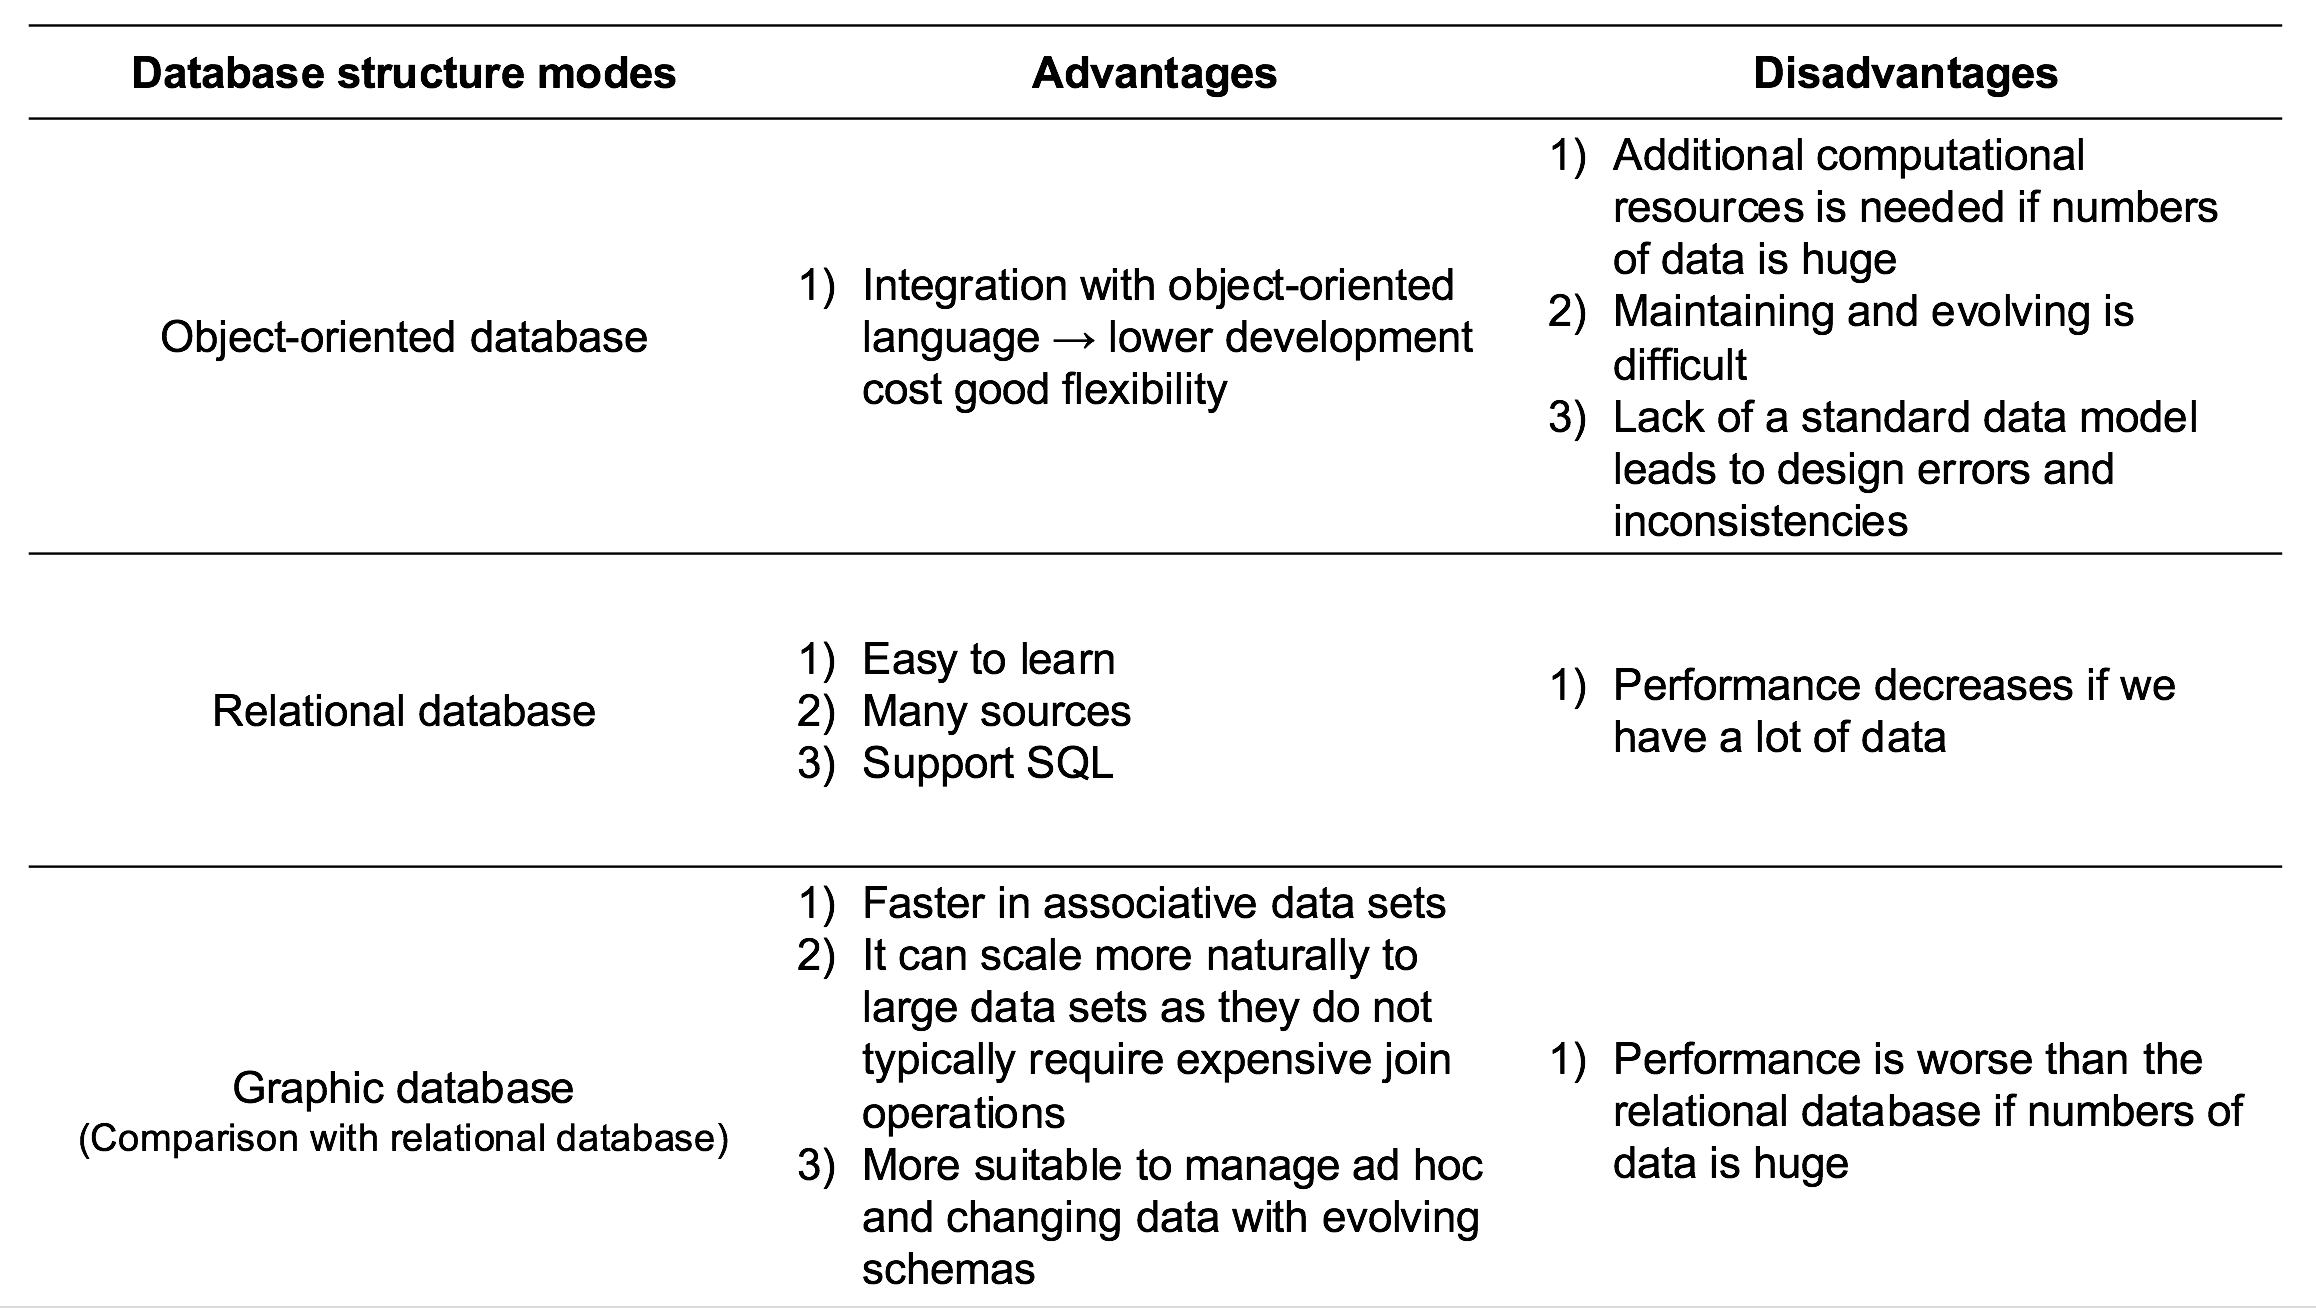
\includegraphics[width=1.8\columnwidth]{Wolverine_Method_Chart_2}
		\end{center}
		\caption{Advantages and disadvantages between three kind of databases.\label{WMC2}}	
	\end{figure*}
	
\end{enumerate}

\subsubsection{SQL and NoSQL}

Every website is full of data, such as Facebook, Bank of Taiwan and official web page of National Cheng Kung University (NCKU).
The database is coming in many forms, including Object-oriented, graph and relational, which are listed above.
Most of the databases come with querying languages interact with databases.
SQL (Structured Query Language) is the most popular among them.
It is also an American National Standards Institute (ANSI) standard.
SQL is a kind of simple language.
It is like English that helps you "communicate" with database server.
Therefore, even the people who are not good at programming can program it easily.


SQL has been a single standard to support all kinds of databases for several decades.
It seems good enough to let us don't need any alternatives.
However, it is going to be changed.
NoSQL is going to be an alternative, which means "non SQL" or "non relational".
It is different from relational database management system (RDMS) in some ways.
For example, NoSQL uses the concept of JSON-like (JavaScript Object Notation) or name-value to store data, instead of using tables like SQL.

However, both SQL and NoSQL have their own advantages and disadvantages.
Therefore, it should be chosen depending on the characteristic of data.
SQL is the ideal language when projects require logical related discrete data that can be identified and data integrity is essential.
On the other hand, NoSQL can be the ideal language if projects require unrelated, indeterminate or evolving data and simultaneously. 
It needs speed and scalability.



\subsubsection{SQLite}
SQLite is an amazing library that gets embedded inside the 
application that makes use of. It also offers an amazing 
set of tools to handle all sorts of data with much less 
constraint and ease. The following data types are supported 
by SQLite: NULL, INTEGER, REAL, TEXT, BLOB. SQLite is file
based which makes it extreme portable and can offer more than 
what is needed for development with the simplicity of working 
with a single file and a linked C based library. Thus, it's 
great for developing and even testing.

\subsubsection{MySQL}
MySQL is the most popular one among the large-scale database servers due to its rich feature and open-source product which powers lots of web-sites and applications online. 
The following data types are supported by MySQL: INTEGER, FLOAT, DOUBLE, DECIMAL, DATE, TIME, CHAR, BLOB, TEXT, ENUM. MySQL is scalable powerful which can handle a lot of data. 
Besides, it has a free community. 
Due to the cross platform, MySQL is a good choice for both development process which works on almost all platforms and for companies with heterogeneous IT infrastructure.
For developers, MYSQL is well known for its efficient workbench tool, admin and data migration which is fast on simple queries.

\subsubsection{PostgreSQL}
PostgreSQL is an open source object-relational database management system (ORDBMS) which has the main goal of being standards-compliant and extensible. 
The following data types are supported by PostgreSQL: boolean, bytea, character, date, double, integer, text, time [(p)], tsquery, xml, and so on. 
Here are the advantages of PostgreSQL.
\begin{enumerate}
	\item It's an open-source SQL and standatd compliant RDBMS. 
	\item It is also adorned with many great and open-source third-party tools for designing, managing and using the management system.
	\item Besides, it has a strong community through which a large amount of knowledge-transfer happens between experienced professional to the amateur developer.
\end{enumerate} 
 

\subsubsection{MongoDB}
MongoDB is an open-source document-oriented database. 
In this case, documents are created and stored in Binary JSON (JavaScript Object Notation) format which enables transferring data between servers and web apps with the use of the human-readable format. 
Besides, MongoDB can store the file as a file system, called Grid file system, 
storing a file into several parts separately, instead of a single document. 
That is why MongoDB can create a load-balance and fault-tolerant system effectively. 
Moreover, the use of dynamic schemas make MongoDB eliminates the need to pre-define the structure. 
Such model allows hierarchical relationships representation, array storage, and ability to change the records structure by simply adding or deleting fields.


\subsubsection{Comparison between four databases}
In comparison with PostgreSQL, there is generally no good reason to use MySQL. 
However there are certain advantages as show in can be found on Figure \ref{CompareDatabase}. which made us to choose PostgreSQL as our database in our project.
PostgreSQL is a relational database. 
It specialists in tracking the relationship between pieces of data and helping you retrieve something if you know something related to it.

\begin{figure*}[htb]
	\begin{center}
		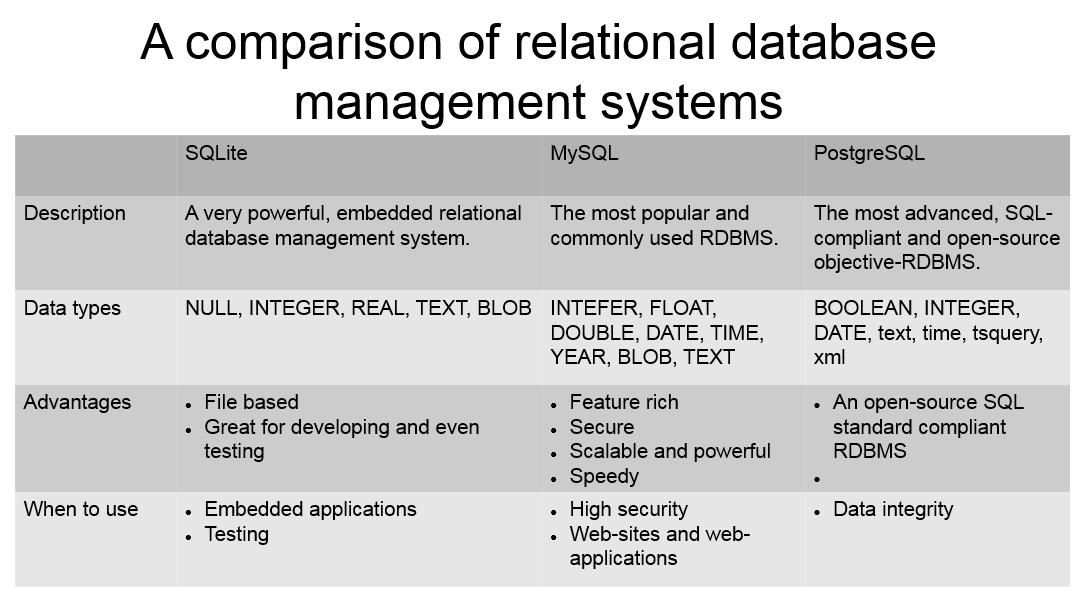
\includegraphics[width=0.8\textwidth]{CompareDatabase}
	\end{center}
	\caption{Comparison between three types of database.\label{CompareDatabase}}
\end{figure*}
\newpage

All SQL databases can do relational queries like this, but PostgreSQL is better at doing this. 
Besides, it also support the data type of "tsquery." which means it can perform full text search.


MongoDB is not a graph database, or even a relational database. 
Like CouchDB, it's a document database and it represents the other end of the scale. 

\subsubsection{Web Crawler}

	
	The web crawler is a program that can automatically browse through web pages, find out the information we assigned and store them.
	It has ability to process the data quickly and accurate to update a very large amount of data which are constantly being updated according to \cite{Liu2012}.
	It starts with a list of URL to visit, called the seeds.
	As crawler visits these URL, it identifies all the informations that we want, such as hyper links in the page and adds them to the list of URL to visit, called the crawl frontier.
	URL from the frontier is recursively visited according to a set of policies.
	If the crawler is performing archiving of websites, it copies and saves the information as it goes.
	The archives are usually stored in such a way they can be viewed, read and navigated as they were on the live web, but are preserved as 'snapshots' from \cite{Du2013}.
	We need to build up a web crawler to automatically visit a list of web page.
	Then find out which link in the page is valuable to download into our database.
	
	

\newpage % Ends the current page and causes all figures and tables to be printed
